Поставим задачу сбор и анализ данных какой"=то группы людей из социальной сети.

В качестве социальной сети идеально подходит <<Вконтакте>>, так как она обладает удобным интерфейсом взаимодействия, а также крайне популярна в РФ. В качестве группы людей выберем  пользователей, подписанных на сообщества <<СГУ Факультет КНиИТ>>, являющаяся основной группой факультата, и <<Душевно>>, которая, в свою очередь, популярна среди студентов факультета.

\subsection{Сбор данных}
<<Вконтакте>> имеет свой собственный API\cite{vk}, с помощью которого можно собрать все необходимые данные. Для начала соберём всех пользователей, подписанных на нужные нам сообщества. Сделать это можно путём отправки запрос на сервер метода \texttt{group.getMembers}. 

Далее для каждого пользователя нам необходимо узнать его ФИО, а также дату рождения, пол и родной город. Стоит отметить, что пользователь может не указать какой"=то из последних трёх параметров или же его скрывать. Для получения данных используется метод \texttt{user.get}. 

После этого соединим пользователей ребром, если они являются друзьями. Воспользуемся методом \texttt{friends.get}, который возвращает всех друзей пользователя. Из них выберем только тех, кто является подписчиком хотя бы одного из выбранных пабликов.

Ознакомиться с кодом, который выполняет все вышеупомянутые функции, можно в приложении \ref{code}.

\subsection{Анализ полученных данных}
Полученные данные конвертируются в два .csv файла, в одном из которых содержится информация каждого пользователя, а в другом "--- связи между ними. Для анализа данных воспользуемся бесплатной программой с открытым исходным кодом "--- <<Gephi>>.

Граф подписчиков состоит из $2401$ вершин и $32208$ ребер.
$54\%$ и $45\%$ подписчиков указали мужской и женский пол соответственно в своём профиле. Лишь $15\%$ всех пользователей указало своим родным городом Саратов, Энгельс или другие города Саратовской области.

\begin{figure}[H]
    \centering
    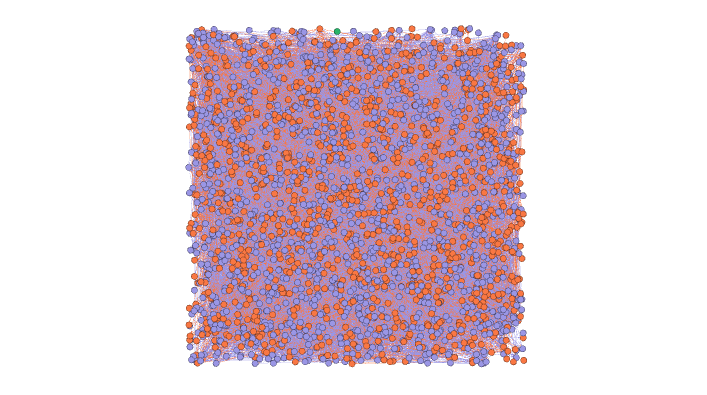
\includegraphics[height = 5cm]{pictures/Graph_without_layout.png}
    \caption{Полученный граф без укладки}
    \label{fig:graph_without_layout}
\end{figure}
Как видим на рисунке \ref{fig:graph_without_layout}, для получения легко читаемого графа необходимо <<раздвинуть>> вершины. Занимается этим различные алгоритмы укладки графа. Воспользуемся алгоритмом Фрюхтермана"=Рейнгольда, относящийся к семейству силовых алгоритмов,в котором используется пружинная физическая модель, где вершины определяются как тела системы, а ребра как пружины.
\begin{figure}[H]
\centering
    \begin{subfigure}[b]{0.3\textwidth}
        \centering
        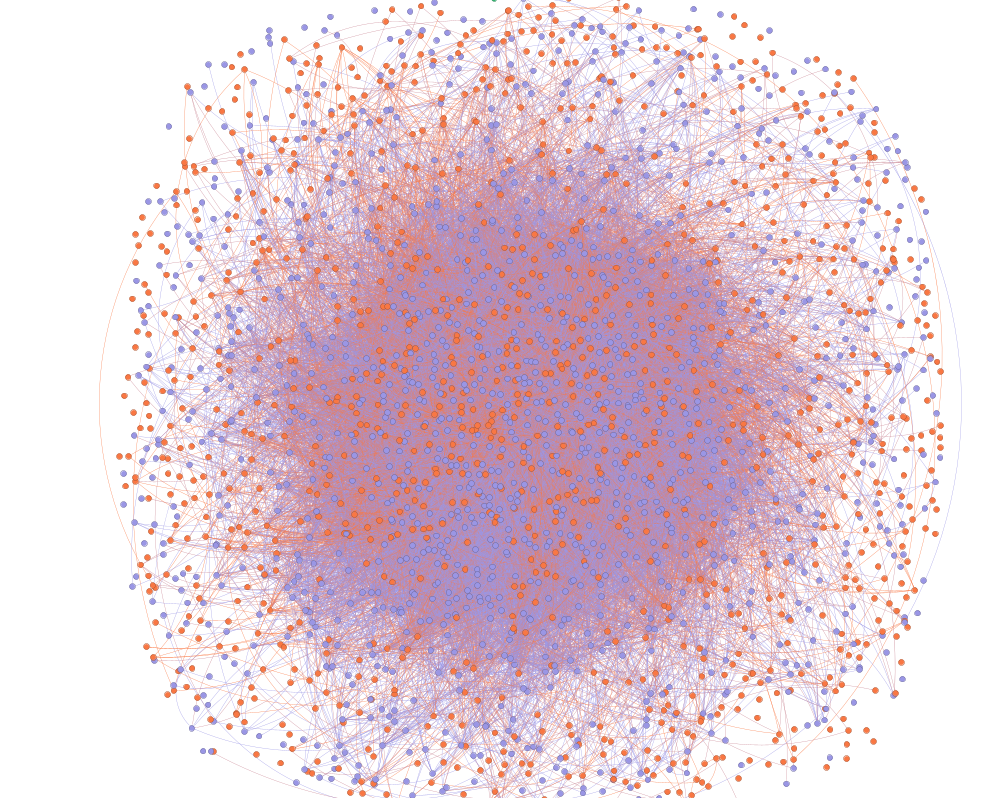
\includegraphics[width = \textwidth]{pictures/Layout_1.png}
    \end{subfigure}
    \begin{subfigure}[b]{0.3\textwidth}
        \centering
        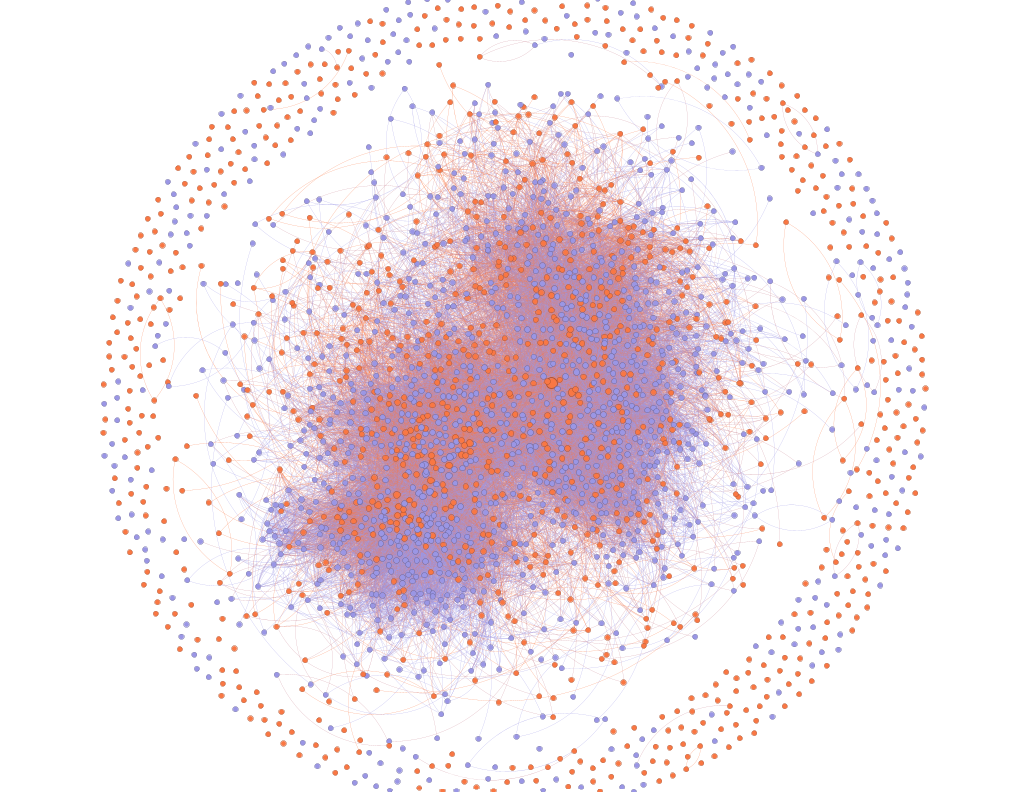
\includegraphics[width = \textwidth]{pictures/Layout_2.png}
    \end{subfigure}
    \begin{subfigure}[b]{0.3\textwidth}
        \centering
        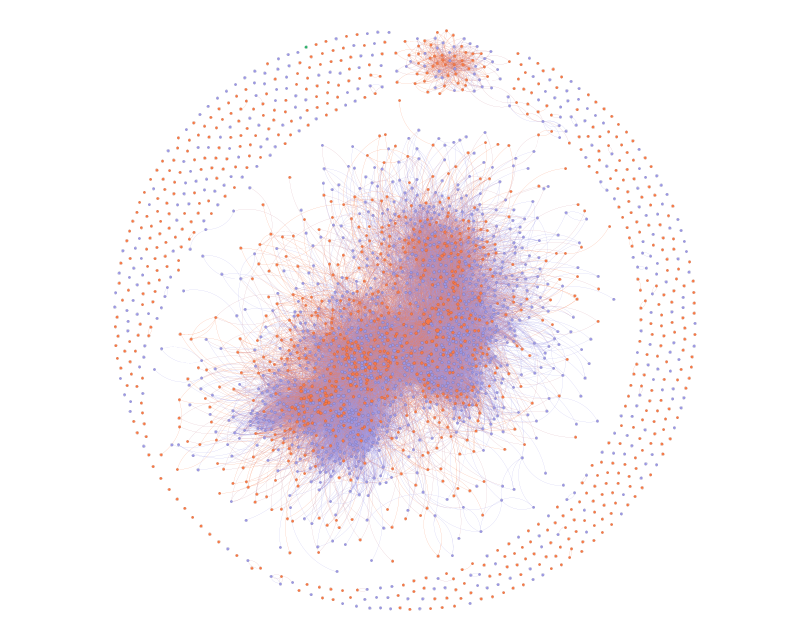
\includegraphics[width = \textwidth]{pictures/Layout_3.png}
    \end{subfigure}
    \caption{Процесс укладки графа}
    \label{fig:graph_layout}
\end{figure}

\begin{figure}[H]
    \centering
    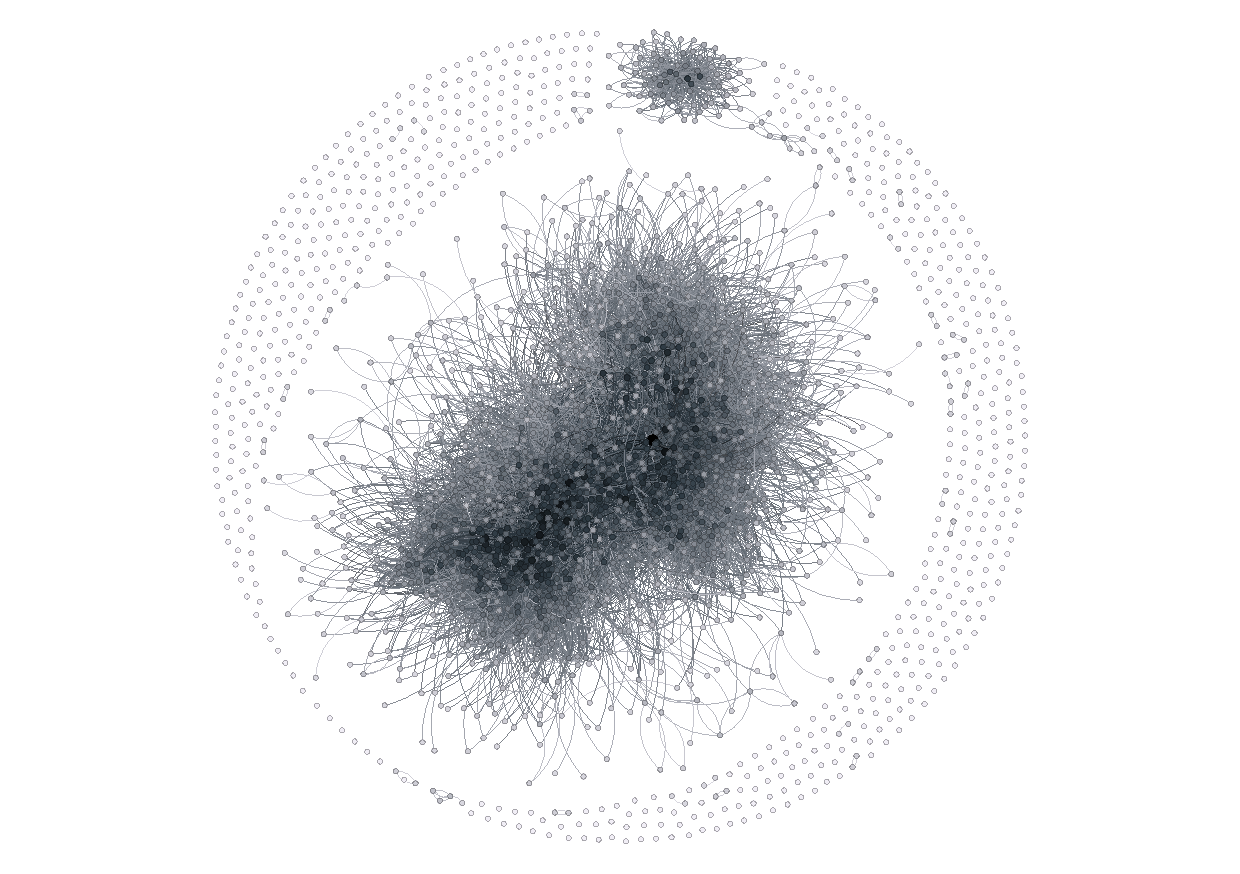
\includegraphics[width = \textwidth]{pictures/Degree Centrality.pdf}
    \caption{Полученный граф после укладки. Применена локальная центральность. Чем темнее вершина, тем больше у неё степень}
    \label{fig:graph_deg}
\end{figure}

Из рисунка \ref{fig:graph_deg} отметим темные вершины, именно они являются самыми общительными среди всех подписчиков.

Кроме того, заметим, что образовался круг из пользователей, который ни с кем не соединены. Вероятно они либо закрыли доступ к своим друзьям, либо являются ботами. Так же заметим, что образовался небольшой круг из пользователей, не связанных с центром. Разобьём граф на компоненты сильной связности для того, чтобы удостоверится в этом.
\begin{figure}[H]
    \centering
    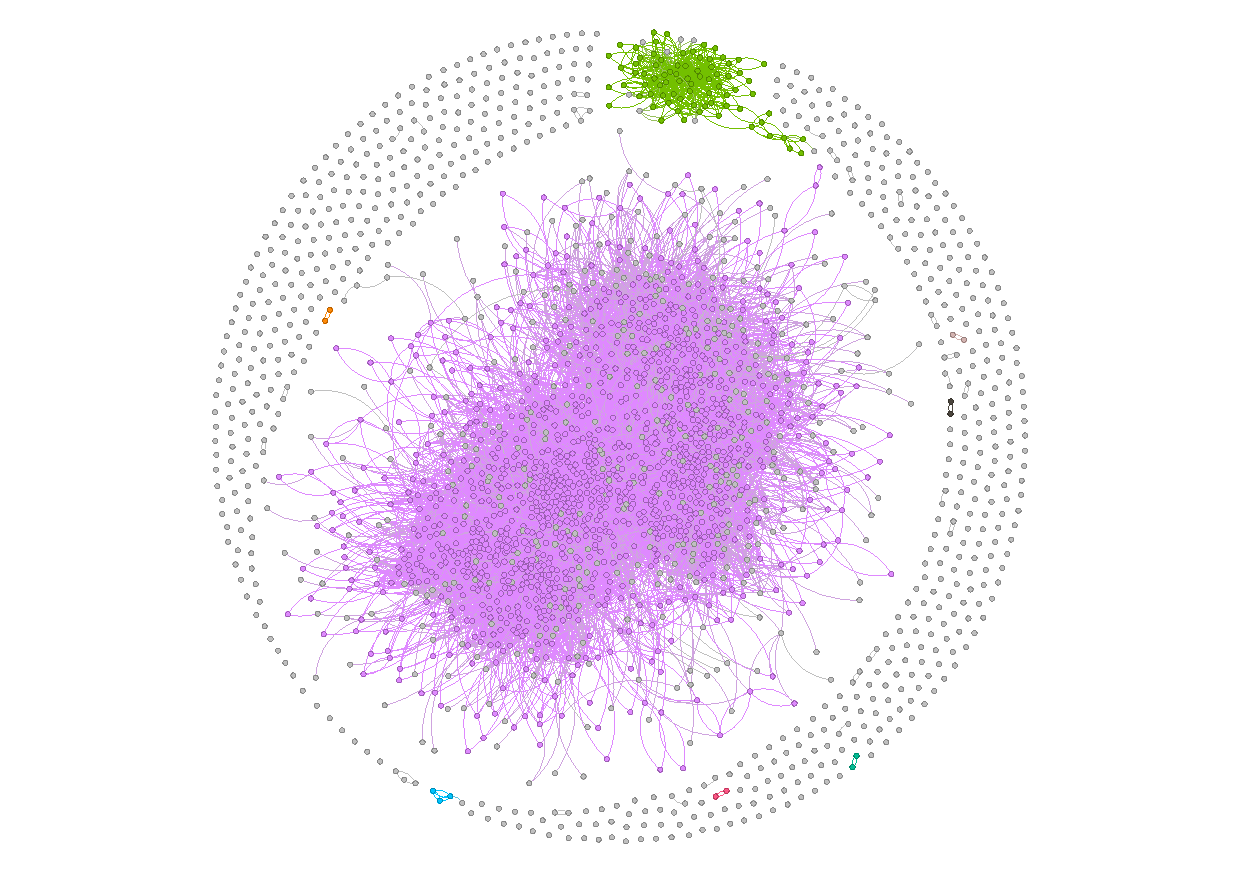
\includegraphics[height = 5cm]{pictures/Strongly component.pdf}
    \caption{Разбиене графа на компоненты сильной связности}
    \label{fig:graph_strong_comp}
\end{figure}
Анализируя <<зелёную>> группу, можно прийти к выводу, что все они являются жителями Санкт"=Петербурга и соответственно никак не связаны со студентами СГУ.

Применим к графу другие центральности:
\begin{figure}[H]
    \centering
    \begin{subfigure}[b]{0.45\textwidth}
        \centering
        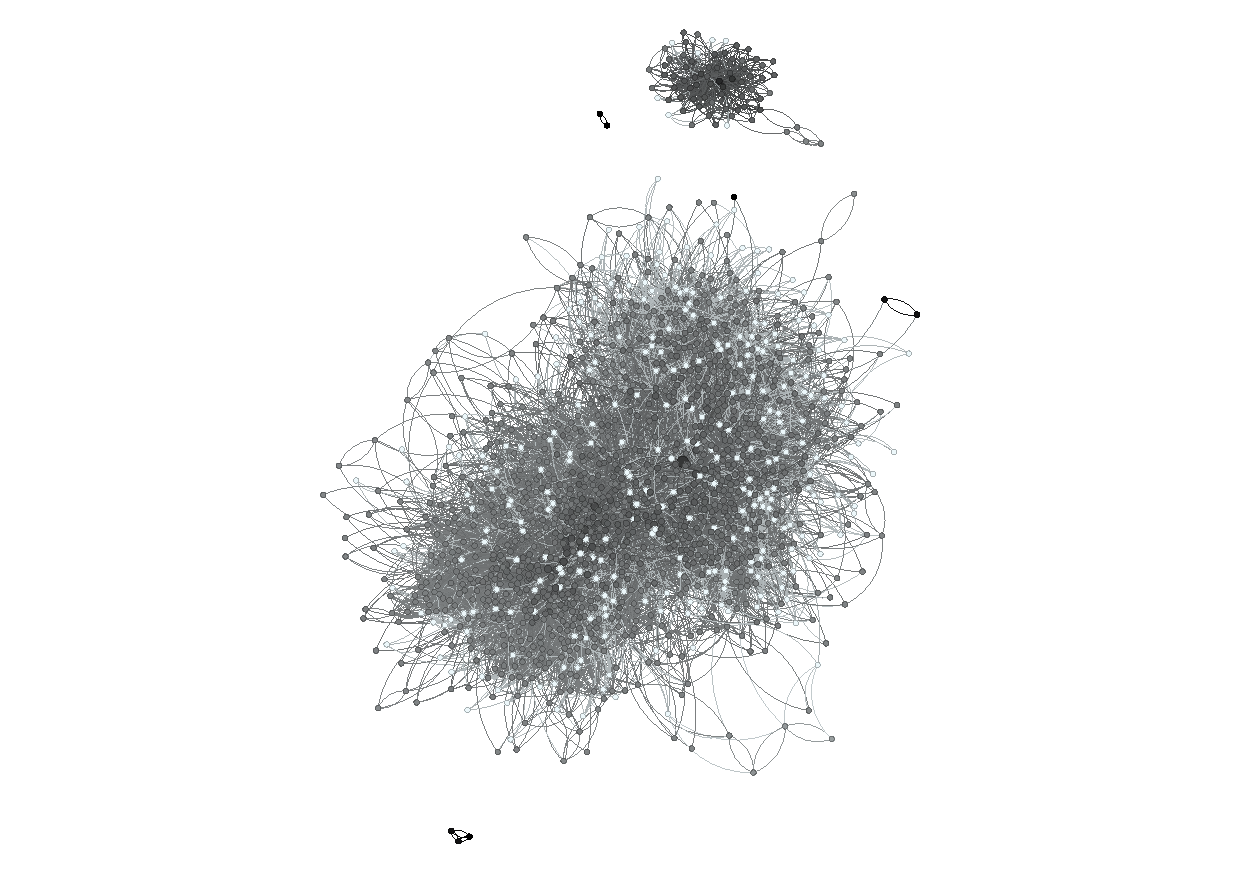
\includegraphics[width = \textwidth]{pictures/Clossenes Centrality.pdf}
        \caption{Степень близости}
        \label{fig:graph_clossenes}
    \end{subfigure}
    \begin{subfigure}[b]{0.45\textwidth}
        \centering
        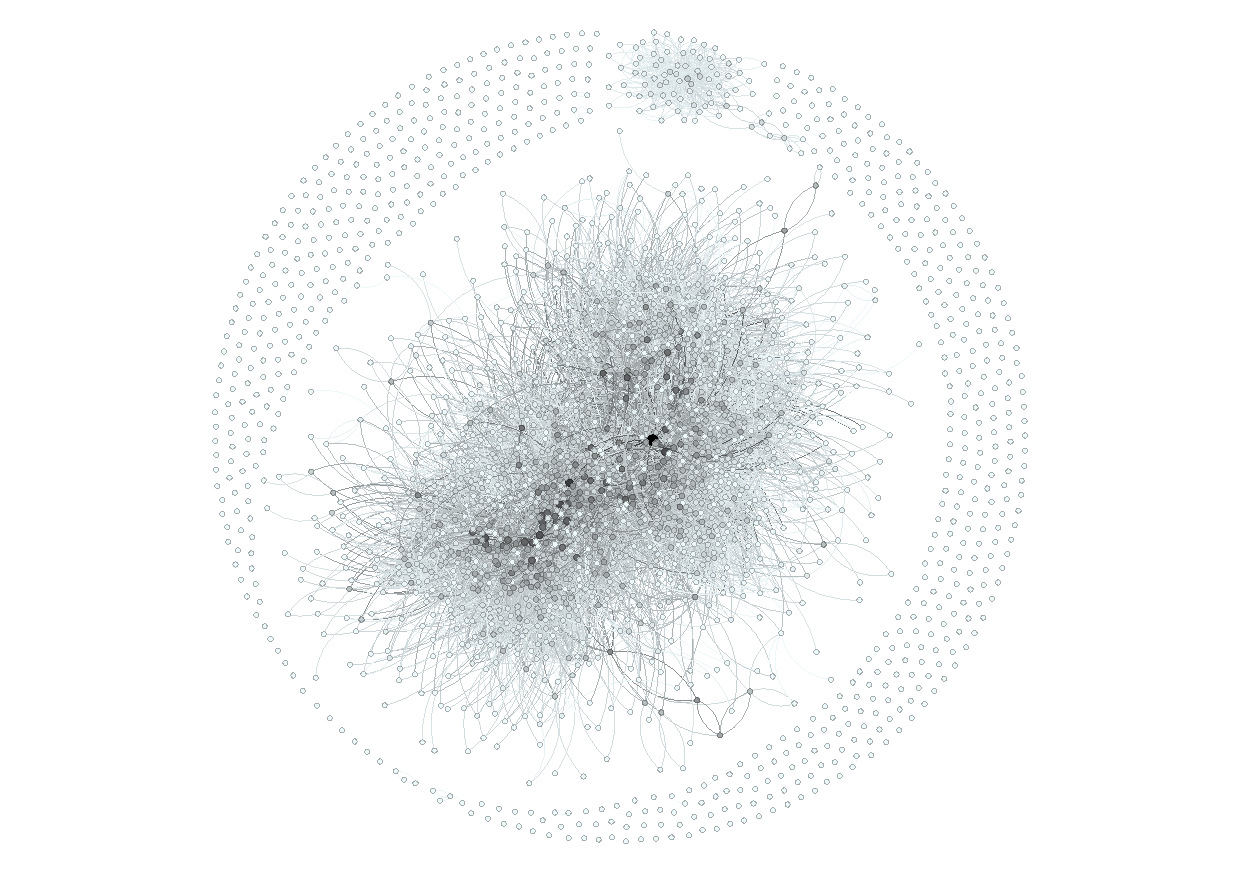
\includegraphics[width = \textwidth]{pictures/Betweenes Centrality.pdf}
        \caption{Степень посредничества}
        \label{fig:graph_betweenes}
    \end{subfigure}
    \caption{Применение к графу других центральностей}
    \label{fig:graph_centrality}
\end{figure}
Посмотрим на рисунок \ref{fig:graph_clossenes}. По нему можно сделать вывод, насколько человек близок к другим, то есть является ли он интровертом или экстравертом.

Обратимся теперь к графу на рисунке \ref{fig:graph_betweenes}, к которому применена степень посредничества. Она показывает, насколько много связей проходит через человека, то есть показывает, насколько он является незаменимым в данном графе.